\section{Experiment}
%===================

Based on the working formula for $\K$, a Gaussian Na\"ive Bayes classifier in Python was created and tested against an \href{https://drive.google.com/file/d/18ZY7I1ym0E9s2ecqjfvmPSGwlXzsNi2n}{\textcolor{blue}{\underline{EMNIST dataset}}} of over 370,000 grayscale 28x28 images of A--Z handwritten alphabets.
\begin{itemize}[noitemsep]
	\item Hence, the dataset has 26 classes (A--Z) with 784 features (pixels) each taking one of 256 values.
	\item The entire dataset was randomly divided into testing sets and training sets in 9:1 ratio.
	\item The classifier uses Gaussian distribution model despite the pixel taking discrete values -- because the training set may not have enough samples to plot the discrete distribution of each pixel accurately.
\end{itemize}
The results of one such experiment are presented in this section:

\subsection{Mean and Variance}
%-----------------------------
The mean and variance of the pixels each alphabet are presented as 28x28 grayscale images. \\
As expected, the mean represents ``what that alphabet on average looks like'', and variance increases towards edges and the `protruding' parts of each alphabet.
\begin{figure}[h]
	\centering
	\caption{Mean of pixel values of each alphabet}\par
	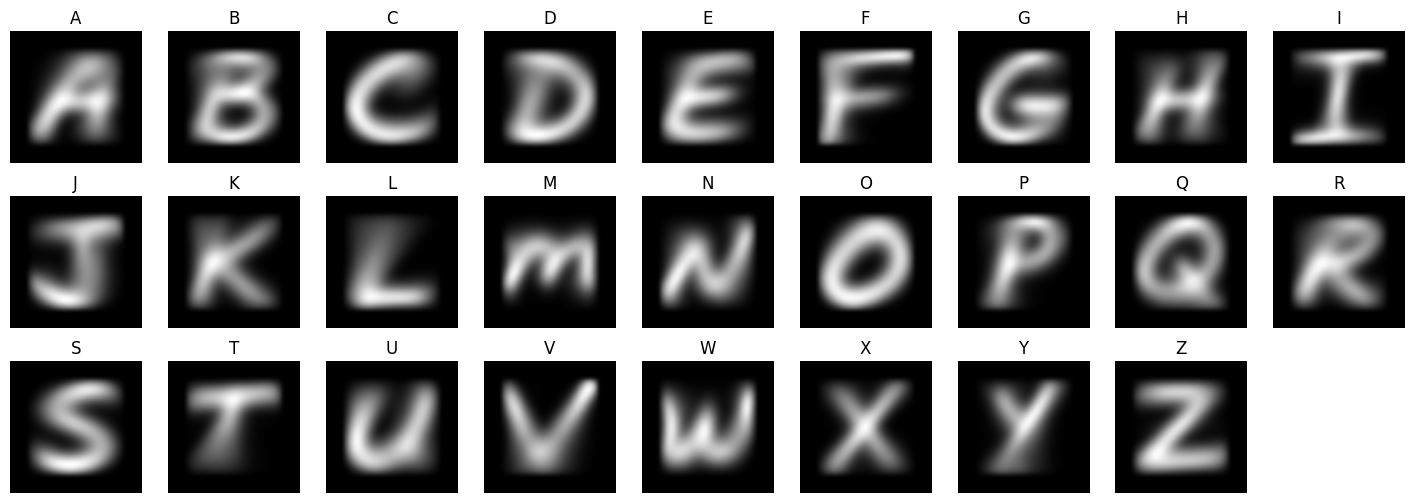
\includegraphics[width=0.9\textwidth]{fig/mean}\par
	\caption{Variance of pixel values of each alphabet}\par
	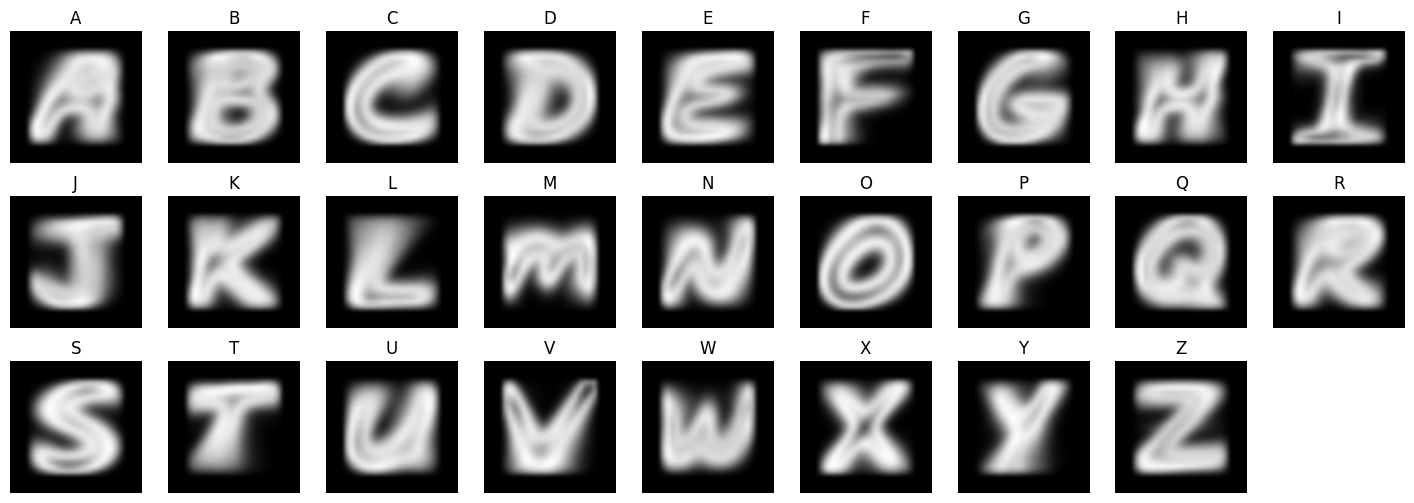
\includegraphics[width=0.9\textwidth]{fig/variance}
\end{figure}

\subsection{Confusion matrix and Accuracy}
%----------------------------------------
As described in section 1, the overall and class-wise accuracy are found using the confusion matrix.
\begin{itemize}[nosep]
	\item Overall accuracy = trace of matrix $\div$ total sum
	\item Class-wise accuracy = value$_{ii}$ $\div$ row-wise sum
\end{itemize}
\begin{figure}[h]
	\centering
	\small
	\caption{Accuracy of prediction}\par
	\textbf{Overall accuracy $\approx 69.82\%$}\par\medskip
	\begin{tabu}{|c|c|c |c|c|c |c|c|c |}
		\tabucline-\rowfont\bfseries
		A        &  B      &  C      &  D      &  E      &  F      &  G      &  H      &  I     \\
		73.27\%  & 70.56\% & 69.11\% & 67.03\% & 56.66\% & 89.81\% & 76.54\% & 44.85\% & 90.62\%\\
		\tabucline-\rowfont\bfseries
		J       &  K      &  L      &  M      &  N      &  O      &  P      &  Q      &  R      \\
		52.82\% & 62.29\% & 72.18\% & 88.65\% & 58.73\% & 83.23\% & 79.27\% & 74.10\% & 45.29\%  \\
		\tabucline-\rowfont\bfseries
		S       &  T      &  U      &  V      &  W      &  X      &  Y      &  Z      & \\
		68.07\% & 70.98\% & 55.90\% & 89.89\% & 79.92\% & 64.53\% & 78.28\% & 52.32\% & \\
		\tabucline-
	\end{tabu}
	\par\bigskip
	\caption{Confusion matrix}\par
	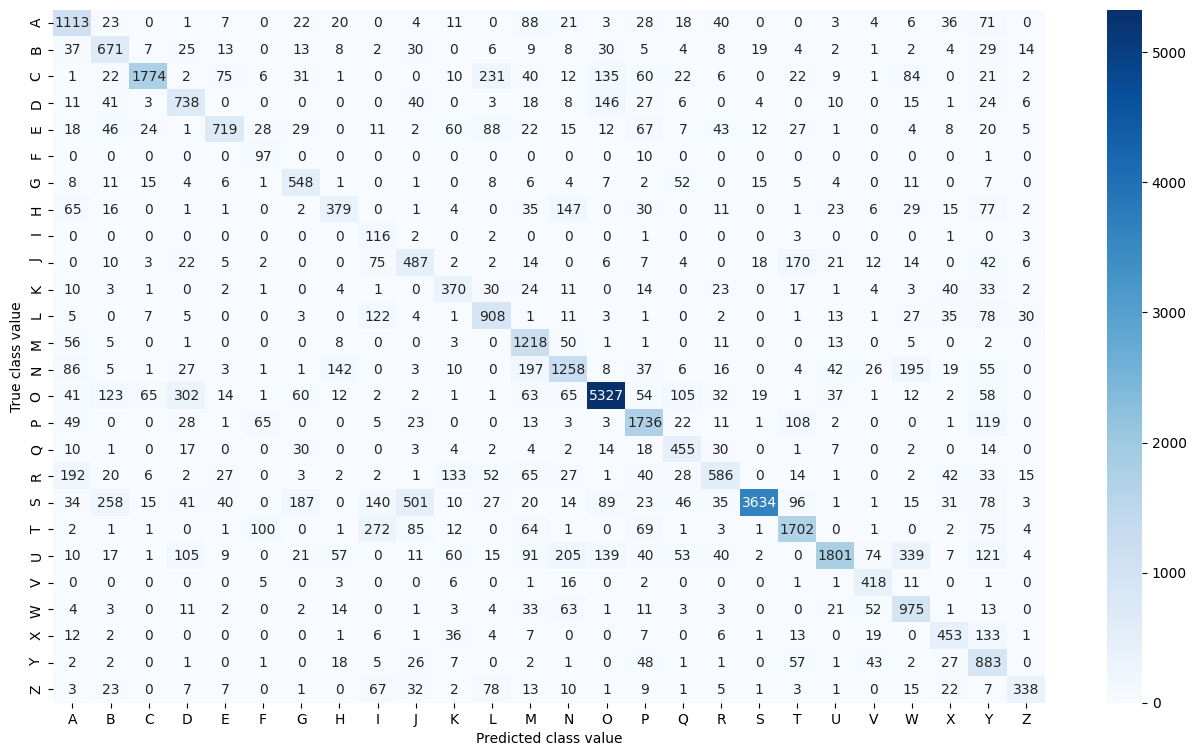
\includegraphics[width=0.8\textwidth]{fig/confusion}
\end{figure}

\textbf{Observations}
\begin{itemize}
	\item Letter `H' has the least accuracy, and is confused for `N' about a third of the time.
	\item Letter `R' has a low accuracy, and is often confused for `A' and `K'.
	\item Letters `F' and `I' seem to have accuracy, but were not tested as much as others.
	\item Letters `O' and `S' were tested the most; letters `I' and `V' have the highest accuracy.
\end{itemize}